\documentclass[11pt]{amsart}
\usepackage{geometry}                % See geometry.pdf to learn the layout options. There are lots.
\geometry{letterpaper}                   % ... or a4paper or a5paper or ... 
%\geometry{landscape}                % Activate for for rotated page geometry
%\usepackage[parfill]{parskip}    % Activate to begin paragraphs with an empty line rather than an indent
\usepackage{graphicx}
\usepackage{amssymb}
\usepackage{epstopdf}
\usepackage[usenames,dvipsnames]{color}
\usepackage{fancyvrb}
\usepackage{listings}
\usepackage{booktabs,footmisc}
\usepackage{hyperref}
\usepackage[all]{hypcap}

\usepackage{topcapt}


 
% include the lines below to use a nicer fixed-width font than the default one
 
\lstset{fancyvrb=true}
\lstset{
	basicstyle=\small\tt,
	identifierstyle=,
	commentstyle=\color{Bittersweet},
	stringstyle=\color{red},
	showstringspaces=false,
	tabsize=3,
	numbers=left,
	captionpos=b,
	xleftmargin=2em
%	numberstyle=\tiny
	%stepnumber=4
	}
\DeclareGraphicsRule{.tif}{png}{.png}{`convert #1 `dirname #1`/`basename #1 .tif`.png}

\title{Repast Java Getting Started}
\author{Nick Collier \& Michael North - Repast Development Team}
%\date{\today}                                           % Activate to display a given date or no date

\begin{document} 
\maketitle
\setcounter{section}{-1}

\section{Before we Get Started}
Before we can do anything with Repast Simphony, we need to make sure that we have a proper installation of Repast Simphony 2.0. Instructions on downloading and installing Repast Simphony on various platforms can be found on the \href{http://repast.sourceforge.net/download.html}{Repast website}.

\section{Getting Started with Repast Simphony for Java}
We will be building a simple agent-based model involving  zombies chasing humans and humans running away from zombies. When we are finished, the running model should look like fig.~\ref{fig:final}.

\begin{figure}[h]
\begin{center}
\vspace{.2in}
\centerline {
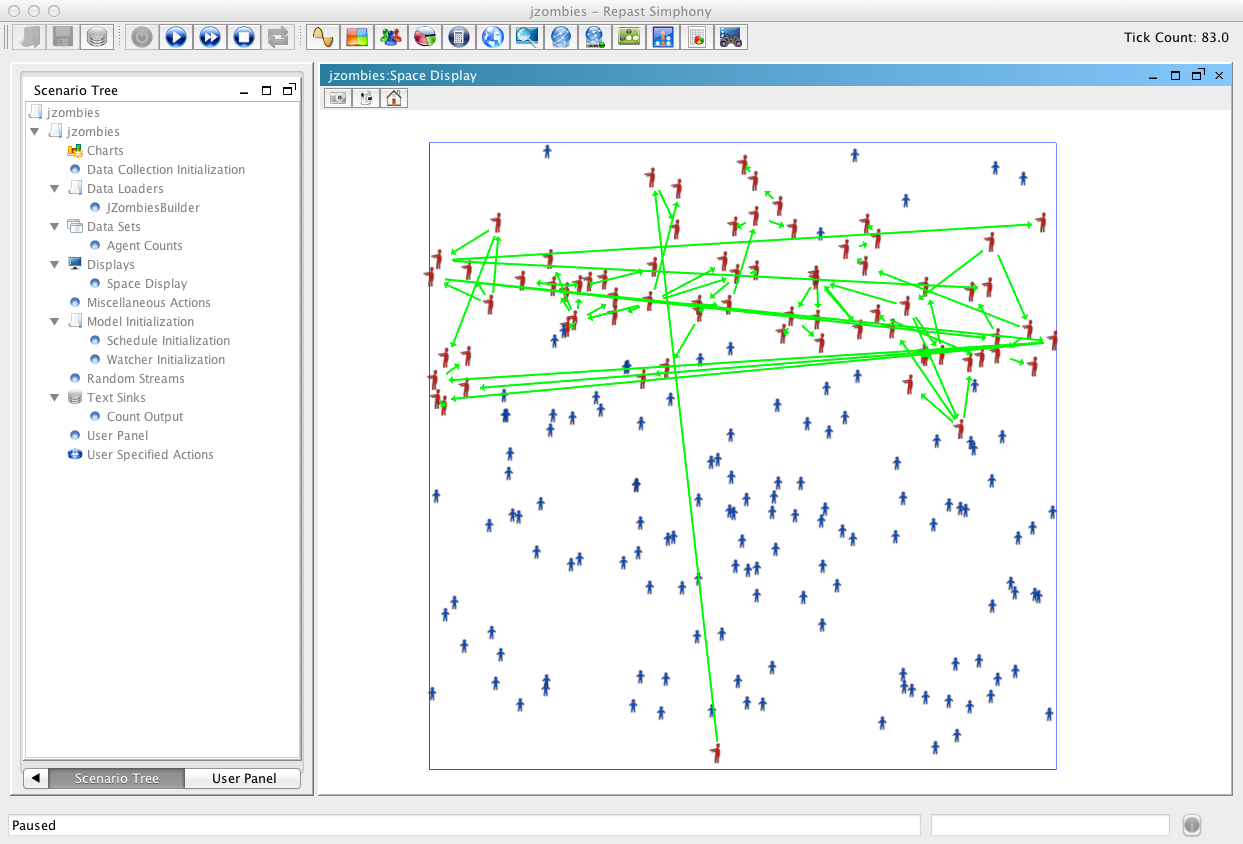
\includegraphics[width=5in]{GettingStartedImages/final.png}
}
\caption{Completed Zombies Model}
\label{fig:final}
\end{center}
\end{figure}

The first thing we must do is create a new Repast Simphony project. Assuming you've started Repast Simphony, right click in the Package Explorer pane and choose ``New'' then ``Other''. A dialog box comes up that allows you to select a wizard. Select ``Repast Simphony Project'' under the ``Repast Simphony'' folder (Fig.~\ref{fig:newprojecticon}) and click ``Next''. This brings up the New Repast Simphony Project Wizard  which gives us the ability to name our project (and a few more options which we'll ignore for now). Type jzombies in the ``Project name" field, and press the ``Finish" button.

\begin{figure}[h]
\begin{center}
\vspace{.2in}
\centerline {
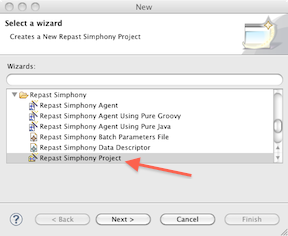
\includegraphics[width=3in]{GettingStartedImages/new_wizard.png}
}
\caption{Repast Simphony Project Wizard.}
\label{fig:newprojecticon}
\end{center}
\end{figure}

 By default Repast Simphony will hide many of the details of the project. This is appropriate for ReLogo projects but not for those written in Java. If the ReLogo filters have not been previously disabled then we need to do that now. If you click on the triangle next to ``jzombies'' and you see a variety of folders (batch, docs, etc), then the filter has been disabled. If you only see the src directory then the filter needs to be disabled. To disable the filter, click the downward pointing arrow in the ``Package Explorer'' pane. If you see ``ReLogo Resource Filter''  then click on it to disable the filter (Fig.~\ref{fig:filter}).  Otherwise, click on the ``Filters'' item. This brings up the Java Element Filters windows. Scroll through the elements and click off the checkbox for ReLogo Resource Filter (Fig.~\ref{fig:filter2}). 


\begin{figure}[h]
\begin{center}
\vspace{.2in}
\centerline {
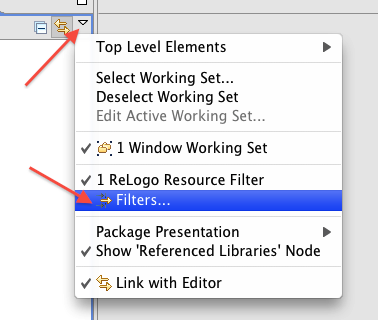
\includegraphics[width=3in]{GettingStartedImages/filter.png}
}
\caption{Disabling the ReLogo Filter.}
\label{fig:filter}
\end{center}
\end{figure}


\begin{figure}[h]
\begin{center}
\vspace{.2in}
\centerline {
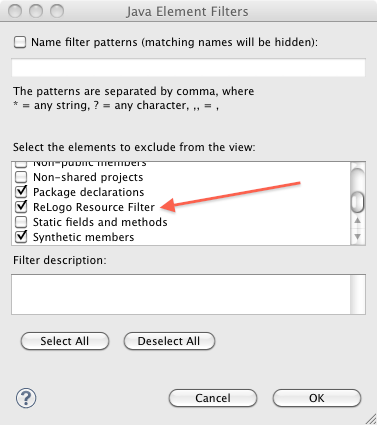
\includegraphics[width=3in]{GettingStartedImages/filter_window.png}
}
\caption{Filter Window.}
\label{fig:filter2}
\end{center}
\end{figure}

Lastly, if eclipse has defaulted to the ReLogo perspective switch it to the Java one. The perspective selections can be found in the upper right hand corner (Fig.~\ref{fig:javap}). Click the Java perspective.

\begin{figure}[h]
\begin{center}
\vspace{.2in}
\centerline {
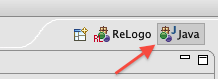
\includegraphics[width=3in]{GettingStartedImages/perspectives.png}
}
\caption{Selecting the Java Perspective.}
\label{fig:javap}
\end{center}
\end{figure}

\subsection{Building the Model}
In a Repast Simphony Java simulation, agents do not need to extend any base class or interface. They can be created simply by using Eclipse's ''New Class Wizard''. The Repast Simphony project wizard creates a source directory and default package into which we can create these agent classes. In our case, the package is ``jzombies'', which can be seen immediately under the src directory.\footnote{Package names typically use an internet domain name as the basis for a package name, but for the purposes of this tutorial ``jzombies'' is perfectly fine. See  \href{http://download.oracle.com/javase/tutorial/java/package/namingpkgs.html}{Java Tutorial: packages} for more info.} The wizard has also created two additional files under the jzombies package: \texttt{ModelInitializer.groovy} and \texttt{ModelInitializer.agent}. These are not necessary for this tutorial and so can be deleted.

\vspace{.2in}
\begin{enumerate}
\item Click on the  \texttt{ModelInitializer.groovy} file
\item Press the delete key on your keyboard. 
\item Repeat for the \texttt{ModelInitializer.agent} file
\end{enumerate}

\vspace{.2in}
We will now create our \texttt{Zombie} and \texttt{Human} classes.
\begin{enumerate}
\item Right click on the jzombies folder under src
\item Click the new class wizard button (Fig.~\ref{fig:class_wizard}).
\item Type Zombie for the name
\item Optionally, click the generate comments box. This won't comment the code for you, of course, but it does
leave a placeholder.
\item Repeat steps 1-4, but type Human for the name of the class
\end{enumerate}

\begin{figure}[h]
\begin{center}
\vspace{.2in}
\centerline {
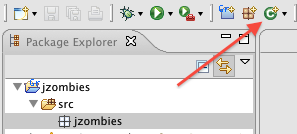
\includegraphics[width=3in]{GettingStartedImages/class_wizard.png}
}
\caption{New Class Wizard Button.}
\label{fig:class_wizard}
\end{center}
\end{figure}

You should now see  \texttt{Zombie.java}  and \texttt{Human.java} files in the jzombies packages underneath the src folder, and these files should be open in Eclipse's editor pane. (If they are not open, double click on each file to open it). Let's begin with the Zombies. The Zombies behavior is to wander around looking for Humans to infect. More specifically, each iteration of the simulation, each Zombie will determine where the most Humans are within its local area and move there. Once there it will attempt to infect a Human at that location and turn it into a Zombie. 

Rather than implementing that all at once, we will begin by implementing the movement. To do this we will locate the Zombies and Humans within a \texttt{ContinuousSpace} and a \texttt{Grid}. A \texttt{ContinuousSpace} allows us to use floating point numbers (e.g. 1.5) as the coordinates of a Zombie's and Human's location, and the \texttt{Grid} allows us to do neighborhood and proximity queries (i.e. ``who is near me?'') using discrete integer Grid coordinates.\footnote{More details on \texttt{ContinuousSpace} and \texttt{Grid} can found in the Repast Java API documentation and the Repast Reference.} Let's begin by adding some field variables and a constructor to the Zombie class. \textbf{Note that copying the text straight from this document may lead to irregular spacing and other issues in the Eclipse editor.}

\noindent\begin{minipage}[h]{\textwidth}
\vspace{.2in}
\lstset{language=java,caption=Zombie Constructor and Variables}
\begin{lstlisting}
public class Zombie {

	private ContinuousSpace<Object> space;
	private Grid<Object> grid;
	
	public Zombie(ContinuousSpace<Object> space, Grid<Object> grid) {
		this.space = space;
		this.grid = grid;
	}
}
\end{lstlisting}
\vspace{.2in}
\end{minipage}

Line 3 and 4 are field variables to hold the space and grid in which the zombie will be located. The Zombie will move about the ContinuousSpace and we will simply round the ContinuousSpace location to determine the corresponding Grid location. Lines 6-9 constitute the constructor which sets the values of the \texttt{space} and \texttt{grid} variables. The \texttt{space} and \texttt{grid} variables have \texttt{Object} as their template parameter. This allows use to put anything in them and prevents Eclipse from giving us spurious warnings. You may need to add the appropriate imports for \texttt{ContinuousSpace} and \texttt{Grid}. These imports looks like:

\noindent\begin{minipage}[h]{\textwidth}
\vspace{.2in}
\lstset{language=java,caption=Zombie Imports}
\begin{lstlisting}
import repast.simphony.space.continuous.ContinuousSpace;
import repast.simphony.space.grid.Grid;
  
\end{lstlisting}
\vspace{.2in}
\end{minipage}
You can add these automatically in Eclipse by right clicking on the type (e.g  \texttt{Grid}) that needs an import and choosing Source - Add Import from the menu. \textbf{As new code is added during the tutorial, you will need to add the appropriate imports. Whenever you see the red squiggle, use Eclipse to add the necessary imports.}\\


Now lets add a method to Zombie that will be called every iteration of the simulation\footnote{Repast Simphony also provides a wizard for adding typical snippets of code. This wizard can be activated using the top hat icon in the Eclipse toolbar. The wizard produces groovy compatible code so some additional work may need to be done to make it Java compatible}.  We will call this method \texttt{step}.

\noindent\begin{minipage}[h]{\textwidth}
\vspace{.2in}
\lstset{language=java,caption=step Method}
\begin{lstlisting}
public void step() {
	// get the grid location of this Zombie
	GridPoint pt = grid.getLocation(this);
	
	// use the GridCellNgh class to create GridCells for 
	// the surrounding neighborhood.
	GridCellNgh<Human> nghCreator = new GridCellNgh<Human>(grid, pt, 
		Human.class, 1, 1);
	List<GridCell<Human>> gridCells = nghCreator.getNeighborhood(true);
	SimUtilities.shuffle(gridCells, RandomHelper.getUniform());
	
	GridPoint pointWithMostHumans = null;
	int maxCount = -1;
	for (GridCell<Human> cell : gridCells) {
		if (cell.size() > maxCount) {
			pointWithMostHumans = cell.getPoint();
			maxCount = cell.size();
		}
	}
}
\end{lstlisting}
\vspace{.2in}
\end{minipage}

Line 3 gets the location of this Zombie (\texttt{this} refers to the object whose method is calling the code) in the grid. We then use a \texttt{GridCellNgh} to create a \texttt{List} of \texttt{GridCell}s containing Humans. A  \texttt{GridCellNgh} is used to retreive a list of \texttt{GridCells} that represent the contents and location of the 8 neighboring cells around a \texttt{GridPoint}. The constructor to \texttt{GridCellNgh} takes the grid whose cells we want to get, the point whose neighboring grid cells we want, the Class of the items we want in the cells, and the extent along the appropriate dimensions. Lines 7 and 8 specify the grid and the location of this Zombie as the point whose neighboring cells we want. By specifying the Human class in the constructor and as a template parameter we filter out any non-Humans. Consequently, our GridCells will on contain Humans. We then call \texttt{getNeighborhood} passing \texttt{true} to it. By passing \texttt{true} the returned list of GridCells will contain the center cell where the Zombie is currently located. Using \texttt{SimUtilities.shuffle}, we shuffle the list of \texttt{GridCells}. Without the shuffle, the Zombies will always move in the same direction when all cells are equal. We use the \texttt{RandomHelper} class to provide us with a random generator for the shuffle. The remaining code iterates through the list of \texttt{GridCell}s and determines which one of them has the largest size. A \texttt{GridCell}'s size is a measure of the number of objects it contains and thus the cell with the greatest size contains the most Humans.

Now that we have discovered the location with the most Humans (i.e. \texttt{pointWithMostHumans}), we want to move the Zombie towards that location. We will first write this method then add the code to call it in the \texttt{step()} method.

\noindent\begin{minipage}[h]{\textwidth}
\vspace{.2in}
\lstset{language=java,caption=moveTowards Method}
\begin{lstlisting}
public void moveTowards(GridPoint pt) {
	// only move if we are not already in this grid location
	if (!pt.equals(grid.getLocation(this))) {
		NdPoint myPoint = space.getLocation(this);
		NdPoint otherPoint = new NdPoint(pt.getX(), pt.getY());
		double angle = SpatialMath.calcAngleFor2DMovement(space, 
			myPoint, otherPoint);
		space.moveByVector(this, 1, angle, 0);
		myPoint = space.getLocation(this);
		grid.moveTo(this, (int)myPoint.getX(), (int)myPoint.getY());
	}
}
\end{lstlisting}
\vspace{.2in}
\end{minipage}

\texttt{moveTowards()} begins with a check to make sure that the Zombie is not already at the location we want to move towards. Then we get the Zombies current location in space as a \texttt{NdPoint}. \texttt{NdPoint} stores its coordinates as doubles and thus it is appropriate when working with \texttt{ContinuousSpace}s. We want the Zombie to move towards the \texttt{GridPoint pt}, but in order to make this sort of movement using a \texttt{ContinuousSpace} we need to convert that \texttt{GridPoint} to a \texttt{NdPoint}. Line 5 does that. We then use the \texttt{SpatialMath} method \texttt{calcAngleFor2DMovement} to calculate the angle along which the Zombie should move if it is to move towards the \texttt{GridPoint}. Line 8 then performs this movement and moves the Zombie in the \texttt{ContinuousSpace} 1 units along the calculated angle. The last two lines update the Zombies position in the \texttt{Grid} by converting its location in the \texttt{ContinuousSpace} to \texttt{int} coordinates appropriate for a \texttt{Grid}.

Once you've written this \texttt{moveTowards()} method, add a call to it in the \texttt{step()} method. The end of the \texttt{step()} should now look like:

\noindent\begin{minipage}[h]{\textwidth}
\vspace{.2in}
\lstset{language=java,caption=Step with MoveTowards Added}
\begin{lstlisting}
for (GridCell<Human> cell : gridCells) {
	if (cell.size() > maxCount) {
		pointWithMostHumans = cell.getPoint();
		maxCount = cell.size();
	}
}
moveTowards(pointWithMostHumans);
\end{lstlisting}
\vspace{.2in}
\end{minipage}
Note the addition of the call to \texttt{moveTowards()} following the for loop.

We want the \texttt{step} method to be called every iteration of the simulation. We can do this by adding an \texttt{@ScheduledMethod} annotation on it. Obviously, the method itself is part of a class, and thus what we are actually scheduling are invocations of this method on instances of this class. For example, if we have 10 Zombies, then we can schedule this method to be called on each of those Zombies. The annotation has a variety of parameters that are used to specify when and how often the method will be called, the number of object instances to invoke the method on, and so on. \footnote{See the Repast Java API documentation and the Repast Reference for more information on the \texttt{@ScheduledMethod} annotation.} 

\noindent\begin{minipage}[h]{\textwidth}
\vspace{.2in}
\lstset{language=java,caption=Step Method with Annotation}
\begin{lstlisting}
@ScheduledMethod(start = 1, interval = 1)
public void step() {
	// get the grid location of this Zombie
	GridPoint pt = grid.getLocation(this);
\end{lstlisting}
\vspace{.2in}
\end{minipage}

The parameters here in line 1 will schedule the step method to be called on all Zombies starting at tick (timestep) 1 and every tick thereafter. 

Let's now turn to the code for the Humans. Select Human.java in Eclipse's editor pane. The basic behavior for a Human is to react when a Zombie comes within its local neighborhood by running away from the area with the most Zombies. Additionally, Humans have  a certain amount of energy that is expended in running away. If this energy is 0 or less then a Human is unable to run. We begin by creating the relevant field variables and constructor.

\noindent\begin{minipage}[h]{\textwidth}
\vspace{.2in}
\lstset{language=java,caption=Human Constructor and Variables}
\begin{lstlisting}
public class Human {
	
	private ContinuousSpace<Object> space;
	private Grid<Object> grid;
	private int energy, startingEnergy;
	public Human(ContinuousSpace<Object> space, Grid<Object> grid, 
		int energy) 
	{	
		this.space = space;
		this.grid = grid;
		this.energy = startingEnergy = energy;
	}
\end{lstlisting}
\vspace{.2in}
\end{minipage}
The Human constructor is identical to that of the Zombie with the addition of \texttt{int energy} and \texttt{startingEnergy}. \texttt{energy} will be used to track the current amount of energy a Human has.  \texttt{startingEnergy} will be used to set the energy level back to its starting level after a Human has had a rest. 

The main behavior of a Human is implemented in its \texttt{run} method.

\noindent\begin{minipage}[h]{\textwidth}
\vspace{.2in}
\lstset{language=java,caption=The Run Method}
\begin{lstlisting}
public void run() {
	// get the grid location of this Human
	GridPoint pt = grid.getLocation(this);
	// use the GridCellNgh class to create GridCells for
	// the surrounding neighborhood.
	GridCellNgh<Zombie> nghCreator = new GridCellNgh<Zombie>(grid, pt,
			Zombie.class, 1, 1);
	List<GridCell<Zombie>> gridCells = nghCreator.getNeighborhood(true);
	SimUtilities.shuffle(gridCells, RandomHelper.getUniform());

	GridPoint pointWithLeastZombies = null;
	int minCount = Integer.MAX_VALUE;
	for (GridCell<Zombie> cell : gridCells) {
		if (cell.size() < minCount) {
			pointWithLeastZombies = cell.getPoint();
			minCount = cell.size();
		}
	}
	
	if (energy > 0) {
		moveTowards(pointWithLeastZombies);
	} else {
		energy = startingEnergy;
	}
}
\end{lstlisting}
\vspace{.2in}
\end{minipage}

This looks much like the Zombie code. A \texttt{GridCellNgh} is used to find the Zombies in the neighboring grid cells. It then determines which of these cells has the least Zombies and attempts to move towards that. Note that \texttt{moveTowards} is only called if the energy level is greater than 0. If energy does equal 0, the Human doesn't move and energy is set back to its starting level. A Human's \texttt{moveTowards} looks like:

\noindent\begin{minipage}[h]{\textwidth}
\vspace{.2in}
\lstset{language=java,caption=}
\begin{lstlisting}
public void moveTowards(GridPoint pt) {
	// only move if we are not already in this grid location
	if (!pt.equals(grid.getLocation(this))) {
		NdPoint myPoint = space.getLocation(this);
		NdPoint otherPoint = new NdPoint(pt.getX(), pt.getY());
		double angle = SpatialMath.calcAngleFor2DMovement(space, myPoint, 
			otherPoint);
		space.moveByVector(this, 2, angle, 0);
		myPoint = space.getLocation(this);
		grid.moveTo(this, (int)myPoint.getX(), (int)myPoint.getY());
		energy--;
	}
}
\end{lstlisting}
\vspace{.2in}
\end{minipage}

This is identical\footnote{We could factor out the duplicate code here to a Zombie and Human shared base class, but for the purposes of this tutorial it is easier to see the code in the class itself} to the Zombie's except that energy is decremented and the human moves 2 units rather than 1.

Unlike the Zombie code we are not going to schedule the \texttt{run()} method for execution. Rather we are going to setup a \textit{watcher} that will trigger this run() method whenever a Zombie moves into a Human's neighborhood. We do this using the \texttt{@Watch} annotation. The \texttt{@Watch} annotation requires the class name of the class to watch, as well as a field within that class. The watcher will trigger whenever this field has been accessed. We can also define a query on the \texttt{@Watch} to further specify when the watcher will trigger.\footnote{See the Repast Java API documentation and the Repast Reference for more details on the \texttt{@Watch} annotation.}  Our \texttt{@Watch} annotation on \texttt{run()} looks like:

\noindent\begin{minipage}[h]{\textwidth}
\vspace{.2in}
\lstset{language=java,caption=Run with Watcher}
\begin{lstlisting}
@Watch(watcheeClassName = "jzombies.Zombie", 
	watcheeFieldNames = "moved", 
	query = "within_moore 1", 
	whenToTrigger = WatcherTriggerSchedule.IMMEDIATE)
public void run() {
\end{lstlisting}
\vspace{.2in}
\end{minipage}

This \texttt{Watch} will watch for any changes to a ``moved" variable in the Zombies class. What this means is whenever any Zombie moves and their moved variable is updated, then this \texttt{Watch} will be checked for each Human. If the query returns true for that particular Human then \texttt{run} will be called immediately on that Human. Our query will return true when the Zombie that moved is within the Moore neighborhood (8 surrounding grid cells) of the Human whose \texttt{Watch} is currently being evaluated.

Sharp-eyed readers will note that we have not defined a ``moved" variable in the Zombie class. So we will do that now. Click on the Zombie editor pane and add \texttt{private boolean moved;} below \texttt{private Grid<Object> grid;}. Then add \texttt{moved = true} to the \texttt{moveTowards} method.

\noindent\begin{minipage}[h]{\textwidth}
\vspace{.2in}
\lstset{language=java,caption=Zombie MovedTowards with Moved}
\begin{lstlisting}
public void moveTowards(GridPoint pt) {
	// only move if we are not already in this grid location
	if (!pt.equals(grid.getLocation(this))) {
		NdPoint myPoint = space.getLocation(this);
		NdPoint otherPoint = new NdPoint(pt.getX(), pt.getY());
		double angle = SpatialMath.calcAngleFor2DMovement(space, 
			myPoint, otherPoint);
		space.moveByVector(this, 1, angle, 0);
		myPoint = space.getLocation(this);
		grid.moveTo(this, (int)myPoint.getX(), (int)myPoint.getY());
		
		moved = true;
	}
}
\end{lstlisting}
\vspace{.2in}
\end{minipage}

That completes this part of the code for Zombies and Humans. Now we need to turn to initializing the simulation. In a Java Repast Simphony model, initialization takes place in a class that extends the Repast Simphony class \texttt{ContextBuilder}. So, let's create one of these now.\\

\begin{enumerate}
\item In the Package Explorer pane, click on the "jzombies" package underneath the src directory. 
\item Click on the "New Java Class" wizard button (Fig.~\ref{fig:class_wizard}).
\item In the Name field, type JZombiesBuilder
\item Click the "Add" button next to the interfaces field
\item Under "Choose interfaces" type ContextBuilder and click OK
\item Click Finish
\end{enumerate}

\vspace{.2in}
An editor pane for \texttt{JZombiesBuilder.java} should now be open. You will notice a red squiggle under the ``T" in \texttt{ContextBuilder<T>} and under \texttt{JZombiesBuilder} in the class declaration. Replace the ``T" with Object to fix the former issue. The error on \texttt{JZombiesBuilder} is because \texttt{JZombiesBuilder} does not implement methods required by the \texttt{ContextBuilder} interface. We can use Eclipse to automatically implement the required methods. Right click on \texttt{JZombiesBuilder}, choose Source then Override / Implement Methods. Click OK on the dialog box that pops up.  (Fig.~\ref{fig:imp}).

\begin{figure}[h]
\begin{center}
\vspace{.2in}
\centerline {
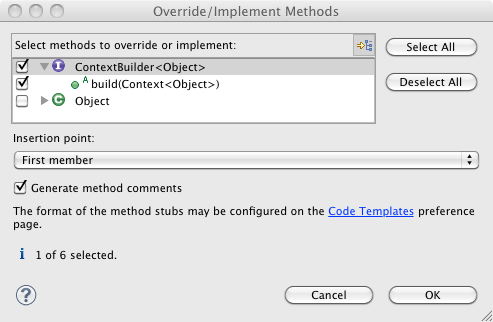
\includegraphics[width=3in]{GettingStartedImages/imp_methods.png}
}
\caption{Override / Implement Methods Dialog.}
\label{fig:imp}
\end{center}
\end{figure}

\noindent\begin{minipage}[h]{\textwidth}
\vspace{.2in}
\lstset{language=java,caption=Skeleton JZombiesBuilder}
\begin{lstlisting}
public class JZombiesBuilder implements ContextBuilder<Object> {

	/* (non-Javadoc)
	 * @see repast.simphony.dataLoader.ContextBuilder
	 	#build(repast.simphony.context.Context)
	 */
	@Override
	public Context build(Context<Object> context) {
		// TODO Auto-generated method stub
		return null;
	}
}
\end{lstlisting}
\vspace{.2in}
\end{minipage}

Your \texttt{JZombiesBuilder} should now look like the above. A ContextBuilder does just what it says it builds a \texttt{Context}. A \texttt{Context} is essentially a named set of agents. Building one consists of naming it, and adding agents to it. Contexts can also have \texttt{Projection}s associated with them. A \texttt{Projection} takes the agents in a \texttt{Context} and imposes some sort of structure on them. Our  \texttt{ContinuousSpace} and \texttt{Grid} are projections. They take agents and locate them in a continuous space and matrix like grid respectively. In \texttt{JZombiesBuilder.build} we are thus going to create the agents and our  \texttt{ContinuousSpace} and \texttt{Grid} projections. Let's begin by initializing the \texttt{Context} and creating the projections.

\noindent\begin{minipage}[h]{\textwidth}
\vspace{.2in}
\lstset{language=java,caption=JZombiesBuilder.build 1}
\begin{lstlisting}
public Context build(Context<Object> context) {
	context.setId("jzombies");
	
	ContinuousSpaceFactory spaceFactory = 
		ContinuousSpaceFactoryFinder.createContinuousSpaceFactory(null);
	ContinuousSpace<Object> space = 
		spaceFactory.createContinuousSpace("space", context, 
			new RandomCartesianAdder<Object>(),  
			new repast.simphony.space.continuous.WrapAroundBorders(), 
			50, 50);
	
	GridFactory gridFactory = GridFactoryFinder.createGridFactory(null);
	Grid<Object> grid = gridFactory.createGrid("grid", context,
	        new GridBuilderParameters<Object>(new WrapAroundBorders(), 
	        new SimpleGridAdder<Object>(),
	         true, 50, 50));
	         
	return context;
}		    
\end{lstlisting}
\vspace{.2in}
\end{minipage}

Note that when doing adding the imports for this code, Eclipse may add the incorrect import for WrapAroundBorders. The correct import should be \newline \texttt{import repast.simphony.space.grid.WrapAroundBorders;} not \\ \texttt{import repast.simphony.space.continuous.WrapAroundBorders}.

We begin in line 1 by setting the id of the passed in \texttt{Context} to "jzombies". Typically, the id should be set to whatever the project name is and should match the context id in the context.xml file (more on this below). The remaining code creates the \texttt{ContinuousSpace} and \texttt{Grid} projections. In both cases, we begin by getting a factory of the appropriate type and then use that factory to create the actual  \texttt{ContinuousSpace} or \texttt{Grid}. Both factories take similar parameters:

\begin{itemize}
\item the name of the grid or space
\item the context to associate the grid or space with
\item an \texttt{Adder} which determines where objects added to the grid or space will be initially located
\item a class that describes the borders of the grid or space. Borders determine the behavior of the space or grid at its edges. For example, WrapAroundBorders will wrap the borders, turning the space or grid into a torus. Other border types such as \texttt{StrictBorders} will enforce the border as a boundary across which agents cannot move.
\item the dimensions of the grid (50 x 50 for example).
\end{itemize}

\vspace{.2in}
The \texttt{GridFactory} differs slightly in that it bundles the borders, adder, dimensions etc. into a GridBuilderParameters object. The \texttt{GridBuilderParameters} also takes a boolean value that determines whether more than object is allowed to occupy a grid point location at a time. With this in mind then, the above code creates a \texttt{ContinuousSpace} named ``space'' and associates it with the passed in \texttt{Context}. Any object added to this space will be added at a random location via the \texttt{RandomCartesianAdder}. The borders of the space will wrap around forming a torus, set via the  \texttt{repast.simphony.space.continuous.WrapAroundBorders()} . Lastly, the dimensions of the space will be 50 x 50. This code also creates a \texttt{Grid} called ``grid" and associates it with the \texttt{Context}. The grid will also wrap and form a torus. Objects added to this grid will be added with the \texttt{SimpleGridAdder} which means that they are not given a location when added, but rather held in a kind of ``parking lot" waiting to be manually added via one of the \texttt{Grid}'s methods. The \texttt{true} value specifies that multiple occupancy of a grid location is allowed. The grid's dimensions will be 50 x 50. Note the we are using the  \texttt{SimpleGridAdder} here so that we can manually set an agent's \texttt{Grid} location to correspond to its \texttt{ContinuousSpace} location. We will do this later in the \texttt{build} method.

Now let's create the agents. Add the following code prior to the return statement.

\noindent\begin{minipage}[h]{\textwidth}
\vspace{.2in}
\lstset{language=java,caption=JZombiesBuilder.build 2}
\begin{lstlisting}
int zombieCount = 5;
for (int i = 0; i < zombieCount; i++) {
	context.add(new Zombie(space, grid));
}

int humanCount = 100;
for (int i = 0; i < humanCount; i++) {
	int energy = RandomHelper.nextIntFromTo(4, 10);
	context.add(new Human(space, grid, energy));
}


\end{lstlisting}
\vspace{.2in}
\end{minipage}

This should be relatively straight forward. We create a specified number of Zombies and Humans by looping through some creation code the specified number of times. We add the new Zombies and Humans to context. In adding them to the context we automatically add them to any projections associated with that context. So in this case, the Zombies and Humans are added to the space and grid using their \texttt{Adders} as described above. The Humans are created with a random energy level from 4 to 10. We use the \texttt{RandomHelper} to do this for us. In general, all random number type operations should be done through the RandomHelper.\footnote{See  RandomHelper in Repast Java API documentation for more information.}

Lastly, we will add the code to move the agents to the \texttt{Grid} location that corresponds to their \texttt{ContinuousSpace} location. The entire \texttt{build} method with this code added follows.

\noindent\begin{minipage}[h]{\textwidth}
\vspace{.2in}
\lstset{language=java,caption=JZombiesBuilder.build Complete }
\begin{lstlisting}
public Context build(Context<Object> context) {
	context.setId("jzombies");
	ContinuousSpaceFactory spaceFactory = 
	ContinuousSpaceFactoryFinder.createContinuousSpaceFactory(null);
	ContinuousSpace<Object> space = 
	spaceFactory.createContinuousSpace("space", context, 
		new RandomCartesianAdder<Object>(),  
		new repast.simphony.space.continuous.WrapAroundBorders(), 
		50, 50);

	GridFactory gridFactory = GridFactoryFinder.createGridFactory(null);
	Grid<Object> grid = gridFactory.createGrid("grid", context,
        		new GridBuilderParameters<Object>(new WrapAroundBorders(), 
        		new SimpleGridAdder<Object>(),
        		true, 50, 50));
	
	int zombieCount = 5;
	for (int i = 0; i < zombieCount; i++) {
		context.add(new Zombie(space, grid));
	}
	
	int humanCount = 100;
	for (int i = 0; i < humanCount; i++) {
		int energy = RandomHelper.nextIntFromTo(4, 10);
		context.add(new Human(space, grid, energy));
	}
	
	for (Object obj : context) {
		NdPoint pt = space.getLocation(obj);
		grid.moveTo(obj, (int)pt.getX(), (int)pt.getY());
	}
	
	return context;
}
\end{lstlisting}
\vspace{.2in}
\end{minipage}

The new code starting at line 28 simply iterates through the all agents in the context, retrieves each one's location in the \texttt{ContinuousSpace} and moves it to the corresponding location in the \texttt{Grid}.

Before we run this model, we need to update the metadata that the Repast Simphony runtime uses to help create displays and other runtime components. Open the jzombies.rs folder under the jzombies project folder, and double click on the \texttt{context.xml} file (fig.~\ref{fig:context}).

\begin{figure}[h]
\begin{center}
\vspace{.2in}
\centerline {
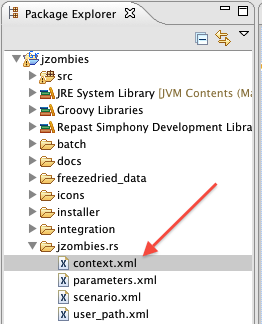
\includegraphics[width=3in]{GettingStartedImages/context_xml.png}
}
\caption{context.xml location}
\label{fig:context}
\end{center}
\end{figure}

That should bring up the xml editor for editing the \texttt{context.xml} file. The \texttt{context.xml} file describes the context hierarchy for your model. The context hierarchy is composed of the contexts your model uses and the projections associated with them. Recall that in our context builder \texttt{JZombiesBuilder} we have a single context and created two projections. We need to update the context.xml to reflect this. By default, the context.xml and editor should have a context already in it with an id of ``jzombies'' (fig.~\ref{fig:cedit1}).

\begin{figure}[h]
\begin{center}
\vspace{.2in}
\centerline {
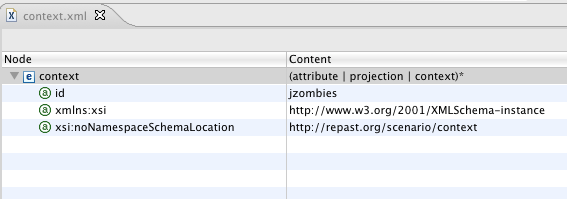
\includegraphics[width=3in]{GettingStartedImages/cedit1.png}
}
\caption{Context.xml editor}
\label{fig:cedit1}
\end{center}
\end{figure}

Note that ``jzombies'' was what we set the context id to in our context builder. We need to add two projections to the xml using the editor, one for the ``grid'' and one for the ``space''. To do that, 
\vspace{.2in}
\begin{enumerate}
\item Right click on the context element and select ``Add Child'' and then ``projection''.
\item Expand the new projection by clicking on the triangle (or plus sign) to the left of it. You should see two attributes
for this projection: type and id.
\item Click in the "content" column for the type attribute and select ``continuous space'' from the drop down box. This sets the value for the type attribute.
\item Next, click in the ``content'' column for the id attribute and type ``space'' (no quotes).
\end{enumerate}

\vspace{.2in}
That adds the metadata for our \texttt{ContinuousSpace} projection. Next let's do the grid.

\vspace{.2in}
\begin{enumerate}
\item Right click on the context element and select ``Add Child'' and then ``projection''.
\item Expand the new projection by clicking on the triangle (or plus sign) to the left of it. You should see two attributes
for this projection: type and id.
\item Click in the "content" column for the type attribute and select ``grid'' from the drop down box. This sets the value for the type attribute.
\item Next, click in the �content� column for the id attribute and type �grid� (no quotes).
\end{enumerate}
\vspace{.2in}

The context.xml editor should now look like Fig.~\ref{fig:cedit2}).

\begin{figure}[h]
\begin{center}
\vspace{.2in}
\centerline {
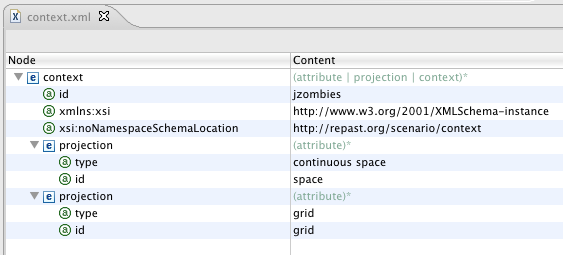
\includegraphics[width=3in]{GettingStartedImages/cedit2.png}
}
\caption{Context.xml Editor Complete}
\label{fig:cedit2}
\end{center}
\end{figure}

Now its time to launch the model. When we created our project using the Repast Simphony Project Wizard, it automatically created Eclipse launchers for us, and we can use those to launch the model. If you click on the small downward facing triangle next to the Eclipse launcher button (fig.~\ref{fig:launch}), you'll see the various available launchers. Click on ``jzombies Model''.

\begin{figure}[h]
\begin{center}
\vspace{.2in}
\centerline {
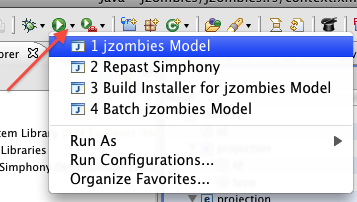
\includegraphics[width=3in]{GettingStartedImages/launcher.png}
}
\caption{jzombies Model Launcher}
\label{fig:launch}
\end{center}
\end{figure}

This will start the Repast Simphony Runtime. Note that you may see some initial errors along the lines of \texttt{SpaceProjectionBuilder - Unable to build continuous space 'space' ...}. These can be ignored for now and in our next steps we are going to correct them. We need to do some runtime configuration before we run the model itself. We are going to setup the runtime to use our context builder to initialize the model and also create an initial display. We setup the runtime to use our context builder by specifying the data loader.

\vspace{.2in}
\begin{enumerate}
\item In the Scenario Tree, right click on the Data Loaders node and click ``Set Data Loader''. If the 
tree is not visible use the tab controls on the left side of the runtime frame to select the Scenario Tree.
\item In the ``Select Data Source Type'' window, click on ``Custom ContextBuilder Implementation''. Click Next.
\item You should see the name of our context builder class in the combo box,\\ \texttt{jzombies.JZombiesBuilder}, if
not,  use the combo box to find it. If the box is empty, go back and check your code. This typically means that there was a compilation error. Click Next.
\item Click Finish.
\end{enumerate}
\vspace{.2in}

You should now see JZombiesBuilder as the name of the Data Loader (fig.~\ref{fig:dl})

\begin{figure}[h]
\begin{center}
\vspace{.2in}
\centerline {
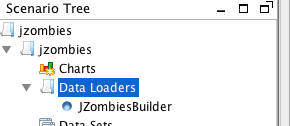
\includegraphics[width=3in]{GettingStartedImages/data_loader.png}
}
\caption{Data Loader}
\label{fig:dl}
\end{center}
\end{figure}

We will now create a simple display. 

\vspace{.2in}
\begin{enumerate}
\item Right click on Displays in the Scenario Tree and click ``Add Display''
\item In the Display configuration dialog, type Space Display for name. Leave 2D as the type.
\item Select our ``space'' projection as the one we want to display. Click on space in the ``Projection and Value Layers'' section and then click the green arrow. The projections on the right are the ones will be displaying and those on the left are all the possible projections to display. The dialog should now look like fig.~\ref{fig:disp1}
\item Click Next.
\item Select the Human and Zombie agents as the types we want to display. Do this by selecting each in the left and then clicking the right pointing arrow to move them to right. If Zombie is not at the top of the list on the left use the up and down arrows to move it to the top. By putting Zombie at the top, the visualized Zombies will be displayed over the Humans if they do overlap.  The dialog should now look like fig.~\ref{fig:disp2}
\item Click Next.
\item In this panel, we can configure what we want the Zombies and Humans to look like. This can be done programmatically by specifying a class that implements \texttt{repast.simphony.visualizationOGL2D.StyleOGL2D} or via a wizard. We will use the wizard to create a simple style for our agents. Click the button to the right of the style class combo box (fig.~\ref{fig:disp3}).
\item In the 2D Shape editor, change the Icon Shape to a square using the combo box and change the color to red by clicking the button with the blue square, and choosing a red color from the icon color dialog. Click OK on the icon color box, then OK on the 2D Shape Editor.
\item Repeat the previous step for the Human. Click on Human in the list of Agents. Then click the icon editor button as before. Leave the default as is, and click OK. 
\item Click Next
\item Click Next
\item Click Finish
\end{enumerate}
\vspace{.2in}

\begin{figure}[h]
\begin{center}
\vspace{.2in}
\centerline {
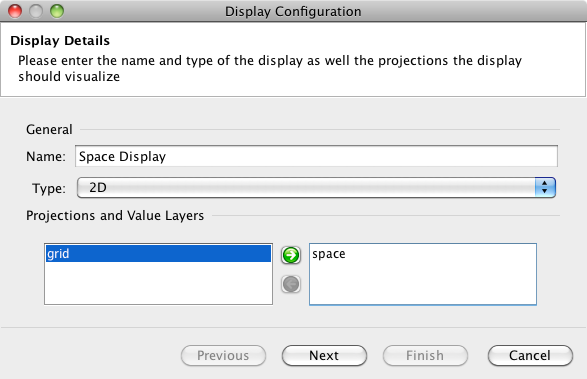
\includegraphics[width=3in]{GettingStartedImages/display1.png}
}
\caption{Configuring the Display}
\label{fig:disp1}
\end{center}
\end{figure}

\begin{figure}[h]
\begin{center}
\vspace{.2in}
\centerline {
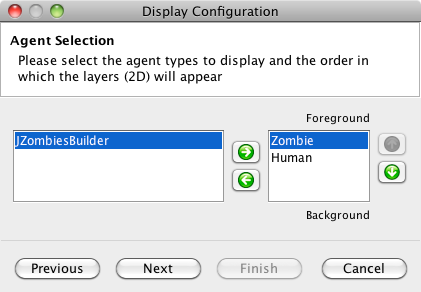
\includegraphics[width=3in]{GettingStartedImages/display2.png}
}
\caption{Configuring the Display 2}
\label{fig:disp2}
\end{center}
\end{figure}

\begin{figure}[h]
\begin{center}
\vspace{.2in}
\centerline {
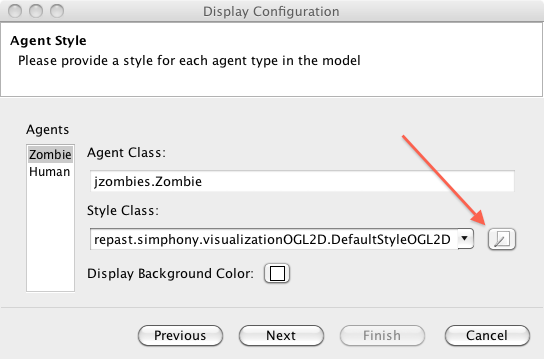
\includegraphics[width=3in]{GettingStartedImages/display3.png}
}
\caption{Configuring the Display 3}
\label{fig:disp3}
\end{center}
\end{figure}

You should now see ``Space Display'' under the Display node in the Scenario Tree. Save your new scenario info (the new Data Loader and Display) by clicking the ``Save'' button (fig.~\ref{fig:save_button}) on the Repast Simphony runtime toolbar.

\begin{figure}[h]
\begin{center}
\vspace{.2in}
\centerline {

\includegraphics[width=3in]{GettingStartedImages/save_button.png}
}
\caption{Save Scenario Button}
\label{fig:save_button}
\end{center}
\end{figure}


We can now run our model. Click the Initialize button (fig.~\ref{fig:buttons}) to initialize the model and bring up the display. If the display is not centered, you can center it by clicking on the display ``home'' button to reset the view. The mouse wheel will zoom the display in and out as will holding down the shift key and right mouse button and moving the mouse up and down. You can run the simulation by clicking the Run button, step through each timestep with the Step button, stop the simulation with the Stop button, and reset it for another run with the Reset button (fig.~\ref{fig:buttons}). When the simulation has been stopped, you must reset it with the Reset button in order do any more runs.

\begin{figure}[h]
\begin{center}
\vspace{.2in}
\centerline {
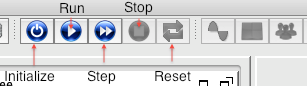
\includegraphics[width=3in]{GettingStartedImages/buttons.png}
}
\caption{Repast Simphony Simulation Buttons}
\label{fig:buttons}
\end{center}
\end{figure}

The display should show 5 red zombie squares and 100 blue human circles. If you repeatedly click the step button  (fig.~\ref{fig:buttons}), you should see the zombies move around. When they do get near a human, the human will move away. Note that a zombie may become stuck in a crowd of humans. This location will be the most desirable place for a zombie and thus the zombie won't move.

Now let's turn back to the code and add some additional behavior. We will now make the Zombies ``infect'' the Humans and turn them into Zombies. We will also add a network projection to model the Zombie infection network. In Eclipse, open the \texttt{Zombie.java} file, if its not already open. If it is open, select it in the editor pane. Let's add a new method to the Zombie class called \texttt{infect}. 

\noindent\begin{minipage}[h]{\textwidth}
\vspace{.2in}
\lstset{language=java,caption=Infect Method}
\begin{lstlisting}
public void infect() {
	GridPoint pt = grid.getLocation(this);
	List<Object> humans = new ArrayList<Object>();
	for (Object obj : grid.getObjectsAt(pt.getX(), pt.getY())) {
		if (obj instanceof Human) {
			humans.add(obj);
		}
	}
	if (humans.size() > 0) {
		int index = RandomHelper.nextIntFromTo(0, humans.size() - 1);
		Object obj = humans.get(index);
		NdPoint spacePt = space.getLocation(obj);
		Context<Object> context = ContextUtils.getContext(obj);
		context.remove(obj);
		Zombie zombie = new Zombie(space, grid);
		context.add(zombie);
		space.moveTo(zombie, spacePt.getX(), spacePt.getY());
		grid.moveTo(zombie, pt.getX(), pt.getY());
		
		Network<Object> net = (Network<Object>)context.
			getProjection("infection network");
		net.addEdge(this, zombie);
	}
}
\end{lstlisting}
\vspace{.2in}
\end{minipage}

In summary, the \texttt{infect()} method gets all the Humans at the Zombie's grid location. A Human is chosen at random from these Humans. The chosen Human is removed from the simulation and replaced with a Zombie. More particularly, the \texttt{infect} method begins by getting the grid location of \texttt{this}, the Zombie calling this code. It then creates a \texttt{List} into which all the Humans at the grid location are put. The loop starting in line 4 iterates through all the \texttt{Object}s at that location, and if they are instances of the Human class it adds them to the list. If the size (the number of elements in the list) of the list is greater than 0 then there are Humans at this location, and we choose one at random. To choose one at random we draw a random number, using RandomHelper, to use as the index into the list. We then get the Object at that index in the list. We get the location in ``space'' of this random human and remove it from the Context. Using the \texttt{ContextUtils} class we get the \texttt{Context} that contains the random human. We then remove it from the context. Removing an object from the context automatically removes it from any projections associated with that context. So, in our case, the random human is removed from the ``space'' and ``grid'' projections. Lastly, we create a new \texttt{Zombie} and add it to the context. Then in line 17, we move it to the random human's location in space using the ``spacePt'' that we retrieved in line 12. We set its grid location to the grid coordinates of this Zombie, using the ``pt'' that we retrieved in line 2. Lastly, we close by getting our infection network by name from the context. (We haven't created this network yet, but will do so shortly.) An edge between \texttt{this}, the Zombie that infected the Human, and \texttt{zombie} is then created.\footnote{See the Java API docs and the user manual for details on working with Network projections}. 

We also need to add a call to \texttt{infect} to the Zombie's \texttt{step} method. Add \texttt{infect()} immediately after \texttt{moveTowards(pointWithMostHumans)} in the \texttt{step} method.

The final step in the code is to create the network in our \texttt{JZombiesBuilder} just as we created the ``space'' and ``grid'' projections. Open \texttt{JZombiesBuilder.java} and add the following to top of the \texttt{build} method. 

\noindent\begin{minipage}[h]{\textwidth}
\vspace{.2in}
\lstset{language=java,caption=}
\begin{lstlisting}
NetworkBuilder<Object> netBuilder = new NetworkBuilder<Object>
	("infection network", context, true);
netBuilder.buildNetwork();
\end{lstlisting}
\vspace{.2in}
\end{minipage}

We use a \texttt{NetworkBuilder} to create the network. This takes a name (``infection network''), the context to associate the network with, and whether or not the network is directed. In our case, we want a directed network with links coming from the infecting zombie to the zombie it created, and so the value is \texttt{true}.\footnote{A \texttt{NetworkBuilder} can build networks from a variety of sources and configurations. See the Java API docs and user manual for details.} In order to actually build the network we then call \texttt{buildNetwork}. This will create the network projection and automatically associate it with the context. Any agents added to the context will then become nodes in this network.

Recall that we had to add ``space'' and ``grid'' to the context.xml file. We now need to do the same for our network. The procedure is the same. Open the \texttt{context.xml} file in Eclipse. Add a new projection element to the context and set its id to ``infection network'' and its type to ``network''. The result should look like fig.~\ref{fig:cxml2}.

\begin{figure}[h]
\begin{center}
\vspace{.2in}
\centerline {
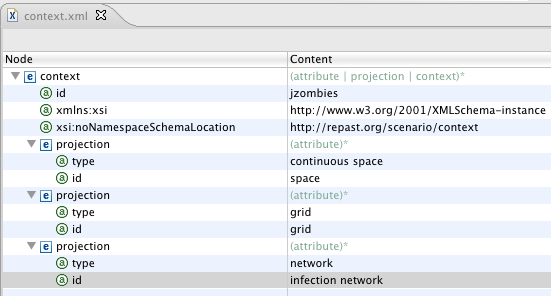
\includegraphics[width=3in]{GettingStartedImages/cxml.png}
}
\caption{context.xml with Network}
\label{fig:cxml2}
\end{center}
\end{figure}

Now let's run our simulation. Start the jzombies Model using the Eclipse launcher as you did before (fig.~\ref{fig:launch}). Once the Repast Simphony runtime has come up, initialize and run the simulation. You should now see humans becoming zombies. If you don't, then check your code for mistakes. Notice that the network is not displayed though. We need to update the display to show the network and in doing so we will also update the styles for the Humans and Zombies. Let's remove the old display first. Right click on the ``Space Display'' in the Scenario Tree under Displays and then ``Delete'''. Now we will make the new display.

\vspace{.2in}
\begin{enumerate}
\item Right click on Displays in the Scenario Tree and click ``Add Display''
\item In the Display configuration dialog, type Space Display for name. Leave 2D as the type.
\item Select our ``space'' and ``infection network'' projections as the ones we want to display. Click on space in the ``Projection and Value Layers'' section and then click the right pointing green arrow. Repeat for the ``infection network''.
\item Click Next.
\item As before, select the Human and Zombie agents as the types we want to display. Do this by selecting each in the left and then clicking the right pointing arrow to move them to the right. If Zombie is not at the top of the list on the left, use the up and down arrows to move it to the top. The dialog should now look like fig.~\ref{fig:disp2}
\item Click Next.
\item In this panel, we can configure what we want the Zombies and Human's to look like. This can be done programmatically by specifying a class that implements \texttt{repast.simphony.visualizationOGL2D.StyleOGL2D} or via a wizard. We will use the wizard to select an icon for our agents. With Zombies selected in the list of Agents, click the button to right of the style class combo box (fig.~\ref{fig:disp3}).
\item In the 2D Shape editor, click on the ``Select Icon File'' button. We want to use the zombie.png icon that comes with the jzombies demo model. Navigate to where the demo models are installed and click on zombies.png in the \texttt{jzombies/icon} directory. (If you can't find zombies.png, feel free to style the Zombie as a circle or whatever, using the 2D Shape editor).
\item Click OK when you have finished.
\item Repeat the previous step for the Human. Click on Human in the list of Agents. Then click the icon editor button as before. Click the``Select Icon File'' button and navigate to the \texttt{jzombies/icon} directory in the demo model. Choose the person.png icon.
\item Click OK when you have finished with the 2D Shape editor.
\item Click Next
\item Click Next
\item Now you can style the infection network. Click the button to the right of the Edge Style Class combo box and then click the button with the black colored square on it to change the edge's color. Click a reddish color and then OK to close the color dialog. Click OK to close the 2D Edge Style Editor.
\item Click Next
\item Click Finish
\end{enumerate}
\vspace{.2in}

You should now see a ``Space Display'' entry under the ``Display'' node in the Scenario Tree. Click the ``Scenario Save''  button (fig.~\ref{fig:save_button}) to save your new scenario configuration.

Run the simulation and you should see the zombies, humans and the zombie infection network. Note that some edges may span the length of the space. Recall that the world is a torus and these edges are in fact between Zombies at the edge of the space. The edge itself can be though of as wrapping  around one side and into the other.

\subsubsection{Data Collection}
Now let's add some data collection to the model. The data we want to record is the number of Zombies and number of Humans at each timestep. Repast Simphony records data from \textit{Data Sources}. The wizard can be used to define Data Sources or you can create them yourself. Data Sources come in two flavors Aggregate and Non-Aggregate. Aggregate data sources receive a collection of objects (agents, for example) and typically return some aggregate value calculated over all the objects. For example, an aggregate data source might call a method on each object and return the maximum value. A non-aggregate data source takes a single object (e.g. a single agent) and returns a value. For example, a non-aggregate data source might call a method on an agent and return the result of that method call. Note that Repast Simphony will take care of which objects to pass to a data source and the actual data collection. You just need to define the data source(s). 

Data collection is setup up in Repast Simphony by defining the data sources described above. These data sources are collected in data sets. Think of a data set as a template for producing tabular data where each column represents a data source and each row a value returned by that data source. To add a data set, 

\vspace{.2in}
\begin{enumerate}
\item Launch the jzombies Model (exit it and relaunch it if it is already running) via the Eclipse launch button.
\item Right click on `Data Sets'' in the Scenario Tree, and click ``Add Data Set''
\item In the Data Set Editor, type Agent Counts as the Data Set ID, and Aggregate as the Data Set type. Recall that we want to 
record the number of Zombies and Humans at each time step. Such counts are considered aggregate operations in that they operate on collections of agents.
\item Click Next
\item In this step, you specify the data sources. The Standard Sources tab allows you to add some standard data sources to your data set. Selecting the tick count check box will create a data source that returns the current tick, the Run Number will return the current run number and Random Seed the current random seed. If the tick count box is not selected, select it now.
\item Click on the Method Data Source tab. The Method Data sources tab allows you to create data sources that will call a method on agents in your model and then perform some aggregate operation on the values returned by that method call.
\item Click the Add button. You should see a row added to the method data sources table that looks like  (fig.~\ref{fig:data1}). Note that the row may not exactly match that of the figure.
\item Double click on the empty table cell in the Source Name column and enter Human Count. 
\item If the Agent Type is not Human, double click on the Agent Type cell and select Human from the drop down list.
\item If the Aggregate Operation is not Count, double click on the Aggregate Operation cell in the table and select Count. The aggregate operation determines what sort of operation is performed on the results of the method call. For example, Min, Max and Mean can be selected here. The Count operation returns the number of objects of the type specified in the Agent Type cell currently in the simulation. No method call is actually applicable here and so that should automatically be set to N/A.
\item Repeat the previous steps beginning with step 7 to add a new row and edit that row to provide a Zombie count. The editor should now look like fig.~\ref{fig:data2}. (The Custom Data Source panel allows you to enter the name of a class that implements either AggregateDataSource or NonAggregateDataSource. We are not using this in this Zombies model.)
\item Click Next
\item The Schedule Parameters panel allows you edit when the data will be recorded. We want to record our data after all the Zombies have moved. Recall that we scheduled the Zombie's \texttt{step} method to start at tick 1 and every tick thereafter. We want to record our data after this. Note that the `Priority'' here is Last which should insure that this records after all the Zombies have moved.
\item Cick Finish
\end{enumerate}
\vspace{.2in}

You should now see an ``Agent Counts'' node underneath the ``Data Sets'' node. \\

\begin{figure}[h]
\begin{center}
\vspace{.2in}
\centerline {
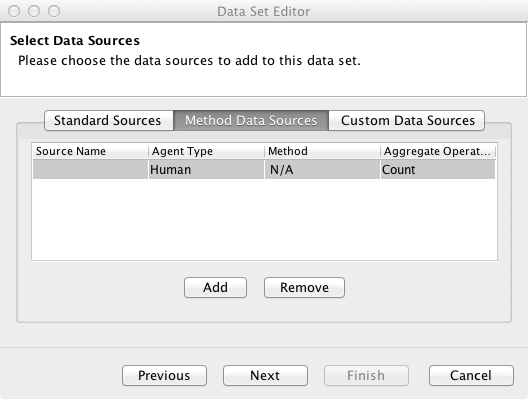
\includegraphics[width=3in]{GettingStartedImages/data1.png}
}
\caption{Selecting Data Sources}
\label{fig:data1}
\end{center}
\end{figure}

\begin{figure}[h]
\begin{center}
\vspace{.2in}
\centerline {
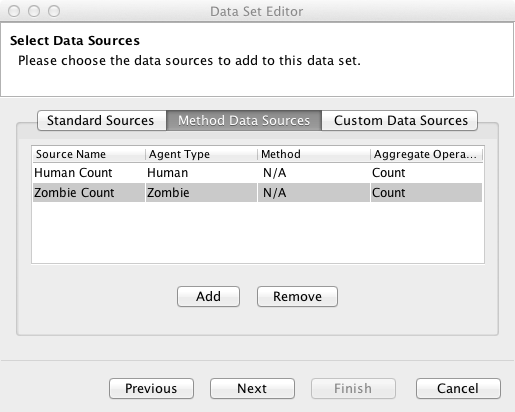
\includegraphics[width=3in]{GettingStartedImages/data2.png}
}
\caption{Selecting Data Sources 2}
\label{fig:data2}
\end{center}
\end{figure}

\subsubsection{Writing Data}

If we run the model now, data will be recorded but we have not set up anywhere for it to be written to.  Simphony can write data to both a file and the console. Console output will show up in Eclipse's console tab and can be useful for debugging. File output will write the recorded data out to a file. We will create some file output by defining a File Sink. 

\vspace{.2in}
\begin{enumerate}
\item Right click on ``Text Sinks'' in the Scenario Tree, and click ``Add File Sink''. 
\item The File Data properties pane allows us to choose what data we want the file sink to write. Enter Count Output as the File Sink name. If we had created more than one data set we might have to choose it from the Data Set Id combo box, but as we didn't the default "Agent Counts" data set is fine. Beneath the Data Set ID box, you will see two columns. The first column lists the data sources associated with the currently selected data set. The second column displays the data sources that will be written to the file. Click on the tick entry in the source list and then click the right arrow button to move it over to the "to-be-written" list. Repeat for the other data sources. You can use the up and down arrows to change the order of the data sources.
\item Click Next
\item The File Properties panel allows us to set some additional file properties: the file name and what meta data to put in the file name. We can leave the defaults as they are. The delimiter specifies what string to use to separate the data values. The format type can be tabular or line. Tabular is the typical CSV spreadsheet table format, while line will precede each data value with the data source name followed by a colon. In our case, this would look something like: tick: 1, Human Count: 20, Zombie Count: 5
\item Cick Finish
\end{enumerate}
\vspace{.2in}

Click the ``Scenario Save''  button (fig.~\ref{fig:save_button}) to save your new scenario configuration. We can now run the simulation and see the output. Initialize and run the simulation for a 100 or so ticks. By default the output will be written to your project directory. In Eclipse, right click on the root jzombies folder in the Package Explorer and choose ``Refresh''. You should now see a file with a name like \texttt{ModelOutput.2010.Nov.19.14\_38\_26\_EST.2.1.txt} in your project directory. If you double click on it you can see the recorded data. (Note that I've justified the text for readability in the listing below.)

\noindent\begin{minipage}[h]{\textwidth}
\vspace{.2in}
\lstset{language=java,caption=Zombie Model Output}
\begin{lstlisting}
"tick",	"Human Count",	"Zombie Count"
1.0,		199,				6
2.0,		199,				6
3.0,		198,				7
4.0,		195,				10
...
\end{lstlisting}
\vspace{.2in}
\end{minipage}

\subsubsection{Creating a Chart} 
We can use the same data set to create a time series type chart that will plot the Human Zombie counts over time. 

\vspace{.2in}
\begin{enumerate}
\item Right click on the Charts entry in the Scenario Tree and select Add Time Series Chart.
\item Enter Agent Counts Chart for the name and choose Agent Counts for the data set. It should be the default if the you have not added any additional data sets.
\item The Chart Data Properties panel allows you to select the data sources to plot in the chart, as well as specify the legend label and color for each data source. Each selected data source will become a series in the chart. Click on the check boxes for the Human and Zombie Count data sources. The default labels and colors are fine (see fig.~\ref{fig:chart1}) but you can change them by double clicking on the label and color entries respectively.
\item Click Next
\item The Chart Properties panel allows you to set the chart's properties. Enter Agent Counts as the title and Number of Agents as the Y-Axis label. The default properties are fine but feel free to change the colors and experiment with the X-Axis range. A range of -1 means the entire range is shown in the x-axis. Anything else restricts the x-axis to displaying the specified range.
\item Click Finish.
\end{enumerate}
\vspace{.2in}

A new Agent Counts Chart should now appear as entry under the Charts tree node. Click the save scenario button to save the chart definition to the scenario. Run the simulation and you should now see a chart displaying the Zombie and Human counts over time.

\begin{figure}[h]
\begin{center}
\vspace{.2in}
\centerline {
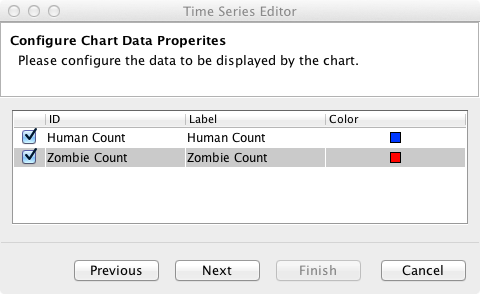
\includegraphics[width=3in]{GettingStartedImages/chart_data.png}
}
\caption{Chart Data Selection}
\label{fig:chart1}
\end{center}
\end{figure}


\subsection{Model Parameters}
Recall that we hard coded the initial number of zombies and humans in our JZombiesBuilder. We shall now convert these to \textit{model parameters}. A model parameter is parameter used by the model that a user can set via the GUI. We can create these in the Repast Simhony Runtime. Launch the JZombies model from eclipse. Use that tabs in panel on the left side of the GUI (where the Scenario Tree is) to select Parameters panel. Click the ``Add Parameter''  button (fig.~\ref{fig:params1}) at the button of the parameters panel. This will bring up the ``Add Parameter'' dialog.

\begin{figure}[h]
\begin{center}
\vspace{.2in}
\centerline {
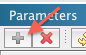
\includegraphics[width=3in]{GettingStartedImages/params1.png}
}
\caption{Parameters Panel}
\label{fig:params1}
\end{center}
\end{figure}

\vspace{.2in}
The  ``Add Parameter'' dialog has the following parts.

\begin{itemize}
\item Name - A unique identifying name for this parameter. Each model parameter should have a unique name.
\item Display Name - The label that will be used in the parameters panel for this model parameter. This does not have to be unique.
\item Type - This can be an int, long, double, or string. You can also add the fully qualified name of any other type.
\item Default Value - The initial value of the parameter.
\item Converter - [Optional] The name of a class that extends\\ repast.simphony.parameter.StringConverter.  A StringConverter can convert non-standard types to and from a String. This is not necessary unless you use a type other than int, long, double, or string.
\item Values - [Optional] A space separated list of values of the chosen type. The parameter will be restricted to these values.
\end{itemize}
\vspace{.2in}

To add our model parameters,

\begin{enumerate}
\item Type zombie\_count for the Name.
\item Type Zombie Count for Display Name.
\item Type int for the Type.
\item Type 5 for the Default Value.
\item Click OK.
\item Click the ``Add Parameter'' button (fig.~\ref{fig:params1}) again.
\item Type human\_count for the Name.
\item Type Human Count for Display Name.
\item Type int for the Type.
\item Type 200 for the Default Value.
\item Click OK.
\end{enumerate}
\vspace{.2in}

The  parameters panel should now look like fig.~\ref{fig:params2}.

\begin{figure}[h]
\begin{center}
\vspace{.2in}
\centerline {
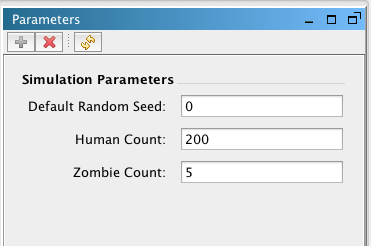
\includegraphics[width=3in]{GettingStartedImages/params2.png}
}
\caption{Parameters Panel With Model Parameters}
\label{fig:params2}
\end{center}
\end{figure}

To use our parameters in our model we need to retrieve them. We can use the \texttt{RunEnvironment} singleton\footnote{See RunEnvironment in the Java API doc for more info.} to get access to the \texttt{Parameters} object. We can then get the parameter's value using \texttt{getValue(String paramName)}. Note that the parameter's value is returned as an Object so we need to cast it appropriately. Make the following changes to JZombiesBuilder.  Replace the hard coded \texttt{zombieCount} value with:

\noindent\begin{minipage}[h]{\textwidth}
\vspace{.2in}
\lstset{language=java,caption=}
\begin{lstlisting}
Parameters params = RunEnvironment.getInstance().getParameters();
int zombieCount = (Integer)params.getValue("zombie_count");
\end{lstlisting}
\vspace{.2in}
\end{minipage}

and the \texttt{humanCount} with:

\noindent\begin{minipage}[h]{\textwidth}
\vspace{.2in}
\lstset{language=java,caption=}
\begin{lstlisting}
int humanCount = (Integer)params.getValue("human_count");
\end{lstlisting}

\end{minipage}

Lauch the jzombies Model, set the parameters and run. Note that the parameters will reset to their default values when the simulation is reset.

\subsubsection{Stochastic Execution and Parameter Sweeps}

Most Repast models use random draws and are therefore stochastic simulations. Stochastic simulations will produce different outcomes for different random number streams, which are generally driven by choosing different random seeds. Such simulations should be executed repeatedly to explore the space of possible outcomes. Even without randomness, model sensitivity analysis parameter sweeps usually should be run to determine the response of the model to changes in input values. Repast provides both local and distributed tools for automatically completing stochastic execution runs and parameter sweeps. Please see the Repast Parameter Sweep Guide for more information.

\subsection{External Tools}

We can also directly connect to some external analysis tools (fig.~\ref{fig:externaltools}). Some of the tools require you, the user, to download addition software and are licensed differently than Repast Simphony. Three of the tools are internal to Repast Simhony and should work out of the box. If you mouse over the buttons themselves, you will see the name of the analysis tool the button refers to. The following analysis tool integrations are available.

\vspace{.2in}
\begin{itemize}
\item MatLab
\item VisAD
\item *ORA
\item R
\item Spreadsheet (Excel by default)
\item Grass (Open Source GIS Software)
\item JUNG (Internal tools that provides some stats on networks)
\item Terracotta
\item Export a Geography Layer to a Shapefile
\item Weka
\item Pajek
\item iReport
\item SQL (Runs SQL like queries on simulation components -- contexts etc.)
\end{itemize}
\vspace{.2in}

We will now experiment with integrating with Excel. Launch the jzombies model again Initialize and run the model for a few hundred ticks.  Click on the Spreadsheets tool plugin button, (the button with the calculator icon). If you have Excel on your machine, chances are the default location is correct. Otherwise select the appropriate location via the Browse button. Click Next and you should see that the File Sink 'Count Output' is selected (Fig.~\ref{fig:spreadsheet}). Click Finish and Excel should launch with the data displayed in a spreadsheet. We recommend experimenting with the various other external tool plugins on your own.

\begin{figure}
\begin{center}
\vspace{.2in}
\centerline {
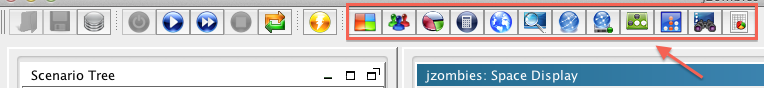
\includegraphics[width=5in]{GettingStartedImages/ExternalTools.png}
}
\caption{The External Tools buttons in the Repast Simphony runtime.}
\label{fig:externaltools}
\end{center}
\end{figure}

\begin{figure}
\begin{center}
\vspace{.2in}
\centerline {
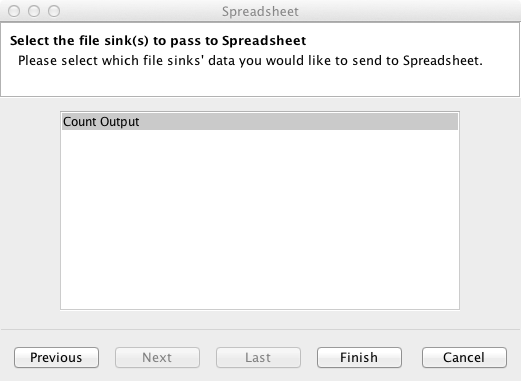
\includegraphics[width=4in]{GettingStartedImages/Spreadsheet.png}
}
\caption{The Spreadsheet wizard with the File Sink selected.}
\label{fig:spreadsheet}
\end{center}
\end{figure}

\subsection{Model Distribution}

Repast models can be distributed to model users via the installation builder. This feature packs up your model and all of the software you need to run it, except for a properly configured Java Runtime Environment, into a single Java archive ("JAR") file that can be given to model users. The resulting installer can be executed on any system with Java version 1.6 or later; JOGL; and Java3D installed\footnote{Users can obtain free JOGL and Java3D files from the Repast website downloads page \href{http://repast.sourceforge.net/downloads.html}{here}.}. Users simply copy the installer file onto their Windows, Mac OS, or Linux computers and the start the installer by double clicking on the file. Once the installer is started it will show an installation wizard that will prompt the user for the information needed to install the model. If desired, the installer can also be run in a command line mode.

Building an installer for a model is straightforward. Simply choose the ``Build Installer for $\langle$Your Model Name Here$\rangle$ Model'' and provide a location and name for the installer file. The installer file's default name is ``setup.jar,'' which is suitable for most purposes. The install builder will then package and compress your model and the supporting Repast software. The resulting installer files are about 70 MB plus the size of the model code and data. 75 MB to 80 MB is a common total size.

The Repast install builder uses the \href{http://izpack.org/}{IzPack system}.  More information on installer customization and use, including command line activation, can be found on the  \href{http://izpack.org/}{IzPack web site}.

\noindent\begin{minipage}[h]{\textwidth}
\vspace{.2in}
\lstset{language=java,caption=}
\begin{lstlisting}

\end{lstlisting}
\vspace{.2in}
\end{minipage}



\end{document}  